%%
%% 研究報告用スイッチ
%% [techrep]
%%
%% 欧文表記無しのスイッチ(etitle,jkeyword,eabstract,ekeywordは任意)
%% [noauthor]
%%

\documentclass[submit,techrep]{ipsj}
%\documentclass[submit,techrep,noauthor]{ipsj}

\usepackage[dvipdfm]{graphicx}
\usepackage{latexsym}
\usepackage{url}

\def\Underline{\setbox0\hbox\bgroup\let\\\endUnderline}
\def\endUnderline{\vphantom{y}\egroup\smash{\underline{\box0}}\\}
\def\|{\verb|}

\setcounter{巻数}{53}%vol53=2012
\setcounter{号数}{10}
\setcounter{page}{1}


\begin{document}

\paffiliate{JU}{愛知工業大学\\
AICHI INSTITUTE OF TECHNOLOGY University}

\title{データベース及び演習 期末レポート\\}

\author{K20089 西宮 銀河}{K20089 Nishimiya Ginga}{IPSJ, JU}[gingin.sol@pluslab.org]

\begin{abstract}
本稿は, データベースおよび演習の授業における最終課題についてのレポートである. 
今回はかんたん備忘録という共有可能なTODOリストを作成した. 機能の詳細は以下より述べる.
\end{abstract}

\maketitle

%1
\section{機能概要}
かんたん備忘録は他の人とノートを共有することができるTODOリストアプリケーションである. 機能としてはシンプルに
備忘録の投稿, 投稿のプライベート化, 自分が投稿した備忘録のチェックを行うことができる. 投稿フォームはスクロールに追従するサイドバーにあるのでどの位置からでも投稿することができる. 
投稿フォームのチェックボックスにマークをつけると投稿がプライベート化され, 最新の備忘録からは確認できなくなるが, マイ備忘録からはいつでも確認することができるので見られたくない投稿はチェックをつけて非表示にすることができる. 

そして新規登録の際はユーザネームと重複防止のためのメールアドレス, そしてパスワードを設定することができる. 
また, これらの項目は必ず入力する必要があり, パスワードは8文字以上, メールアドレスはメールアドレスの形式のみというバリデーションの制限がある. 

登録情報はログイン後サイドバーのリンクから変更することができる. 入力フォームにはユーザデータが取り込まれて表示される.


%2
\section{利用技術}

%2.1
%この節における参考文献
%https://www.php.net/manual/ja/faq.general.php
%http://php.adamharvey.name/manual/ja/internals2.ze1.zendapi.php
%https://www.phptutorial.net/php-tutorial/what-is-php/
\subsection{PHP}
PHPとは"PHP:Hypertext Preprocessor"の略で, 直接HTMLに埋め込んで使用することができる汎用プログラミング言語である. 
構文はC言語, Java, Perlから派生しており, それに加えてPHP独自の構文を組み込むことでPHP特有の機能を使用できる. 
PHPはサーバサイド言語であるので, 主にWebサーバ側で動作する. 
なのでクライアント側からブラウザがHTTPリクエストを送ったとすると, サーバ側がPHPを処理して生成されたHTML文書などをクライアント側に返すという仕組みとなっている. 
そしてPHPはクロスプラットフォーム言語なのでLinux, Windows, MacOSはもちろん, NginXやApacheなど全てのwebサーバ, さらにMicrosoft AzureやAmazon AWSなどのクラウド環境にも対応している. 

また現在の最新バージョンはPHP 8であり, これはZend Engine 4というPHPの実行エンジンの最新バージョンを使用している. これによってオブジェクト指向プログラミングの機能が使えるようになっている. 

%2.2
%この節における参考文献
%https://kinsta.com/jp/knowledgebase/what-is-mysql/
%https://mariadb.org/
%https://www.integrate.io/jp/blog/mariadb-vs-mysql-everything-you-need-to-know-ja/#what
\subsection{MariaDB/MySQL}
まず, MySQLは1995年に開発されたオープンソースソフトウェアのリレーショナルデータベースである. 
'95年以降は所有者も管理者も転々と変わっていたが2010年に所有権がOracle社に移るが, 所有権が渡った今でもオープンソースであることは変わっていない.

MySQLはリレーショナルデータベースと呼ばれるデータの保存方法が使われている. リレーショナルデータベースとは1つのテーブルに全ての情報を挿入するのではなく, 複数のテーブルに分けてそれぞれを関連づけて管理する方法である. 
例えば名前や住所などの顧客データと購入製品や価格などの注文データを扱うテーブルを作るとすると, もし一つのテーブルに全てのデータを入れておくとなった際にデータの重複やデータ削除時の混乱が起こり, 検索が難しくなる. その問題に対処するためにリレーショナルデータベースでは
キーと呼ばれるユニークなIDを利用して異なるテーブル同士を繋げ, データの取り出しや削除などが容易になっている. 

そして, MariaDBはこのMySQLをベースに作られたデータベースである. MySQLと比べてパフォーマンス, 安定性, 開示性が高く, もっとも有名なリレーショナルデータベースの一つとされている. MySQLとの完全な互換性, GPLの採用, さらには開発者コミュニティが豊富なのでMariaDBはMySQLの上位互換と言える. 
%2.3
%この節における参考文献
%https://developer.mozilla.org/ja/docs/Web/CSS
\subsection{CSS}
CSSとは"Cascading Style Sheets"の略で, HTMLやXML文書の見栄えなどを整えるために使われるスタイルシート言語である. 
HTML内で指定されたタグやidなどをセレクタで指定して色や段落などの設定ができる. 

%2.4
%この節における参考文献
%https://www.tutorialspoint.com/laravel/laravel_overview.htm
\subsection{Laravel}
LaravelはMVC方式のPHPフレームワークである. 図 1 に示すようにプロジェクトファイルをデータベースと接続するモデル, HTML 表示を行うためにクライアントにレ スポンスを返すビュー, これらモデルとビューをつなぐコ ントローラの3 つの役割に分けることでフロントエンドとバックエンドそれぞれの開発がしやすくなっている. CodeIgniterやYiiなどのPHPフレームワークやRuby on Railsなどのプログラム言語の基本的な機能を組み込んでいるので豊富な機能が使用できることが特徴である. 
なのでスクラッチ開発でもセキュリティ対策などが簡単に実装できるので容易にWeb開発に取り組むことができる. 
さらにvue.jsなどの他のフレームワークからコンポーネントを持ってくることも可能なのでよりWebアプリケーションの開発が容易になっている.

またLaravelにはプロジェクトの操作に便利なArtisanコマンドというものが搭載されている. このコマンドはSymphonyというフレームワークを使って作られており, これを使用してデータベースの操作, ローカルサーバの立ち上げ, モデル・ビュー・コントローラの生成が簡単にできるようになっている. 

さらにプログラムからデータベースに楽にアクセスするためにEloquentと呼ばれるORM(Object Relational Mapper)が組み込まれている. これによって関数やモデルクラスの使用でSQLの操作が可能となっている.

またビューではbladeと呼ばれるLaravel独自のテンプレートファイルが使用可能で, これを使用することでphpファイル内で条件に応じた処理や別ファイルの継承などを行って便利に表示をさせることができる. 

\begin{figure}[h]
 \centering
 \includegraphics[scale=0.17]{laravel.eps}
\caption{MVCの動作}
 \label{MVC}
\end{figure}


%https://developer.mozilla.org/ja/docs/Web/HTTP
\subsection{HTTP}
HTTPとは"Hypertext Transfer Protocol"の略でハイパーテキストを転送するためのアプリケーション層プロトコルである. 
主にサーバ側とクライアント側との通信の目的のために使われるが別の用途でも使用されることがある. 基本的な動作としてはクライアント側がサーバ側にリクエストを送信するためにポートを開き, サーバ側からレスポンスが帰ってくるまで待機するという仕組みとなっている. 
また, HTTPは主にTCP/IP層の上の通信で使用されるが, UDPのようなトランスポート層でも使用されることがある. 

%3
\section{システム設計}
\subsection{システム概要}
Laravelを使用して3つのコントローラ, 2つのモデル, 11のビューによって構成されている. 

SimpleNoteControllerクラスは主に特にデータベースとの連携などを行わない処理の際に呼び出されるコントローラである. 
ここではトップページの表示, 新規登録の確認画面の表示, ログアウトなどでセッションの操作を行うことがほとんどである. 

次にUserControllerクラスである. ここではユーザデータの操作を行っており, 新規登録の完了, ログイン情報のチェック, 登録情報の編集が機能となっている. またデータベースにユーザデータを挿入する際のパスワードのハッシュ化もここで行っている. 

最後にNoteControllerクラスである. ここでは備忘録の操作を行っている. トップページでの表示の際にidの降順にペジネーションしての表示, 備忘録の投稿, マイページでの表示が主な機能となっている. さらにプライベート投稿であるかのチェックもここで行っており, プライベート投稿であればフラグを立てたものをデータベースに登録している. 
そして備忘録を表示する際にはビュー側でこのフラグを検知して非表示にするかを判断している. 
また, これらUserControllerとNoteControllerはバリデーションもここで行っており, それぞれに独自のRequestクラスを実装してリクエストが渡された際にクラスの機能に応じたバリデーションを行うことでユーザ入力のルール違反をチェックしている. 主にパスワードは8文字以上, 投稿文字数は400文字以内などのルール設定がここで行われ, チェックされている.

そしてモデルはUserモデルクラスとNoteモデルクラスがあり, それぞれUserモデルがNoteモデルの主テーブルであることの宣言やデータベース挿入時のバリデーションなどの関数が搭載されている. 

\subsection{画面遷移}
本システムの画面遷移図は図2のようになっている. まずトップページでは未ログインの状態ではサイドバーは投稿フォームとログインボタン, 既ログインの状態では投稿フォームとマイページ, 登録情報編集, ログアウトへのリンクが設置されている. それ以外はどちらも備忘録の表示のみで同じ構成となっている.
ログインの際にはメールアドレスとパスワードの入力フォームが設置されている. ここにログイン情報を入力することでログイン状態になることができる. またデータが不十分であったり, 登録データが存在しない場合はエラー表示がされる. 

新規登録画面では投稿の際に表示されるユーザネーム, 一意の識別のために使用されるメールアドレス, パスワードの設定を要求される. これらも条件を満たしていないとエラー表示がされ, 満たしている場合は確認画面でチェックを促したのちに登録完了となり, ユーザデータがデータベースに挿入される. ログイン後は設定したユーザネームが投稿フォームに表示される. マイ備忘録ではログインしたユーザの自分の投稿を見ることができる. そして登録情報変更では新規登録画面と同じフォームで登録した情報を変更することができる. 

備忘録の投稿においては未ログインであれば名無し, 既ログインであれば登録時のユーザネームを使って投稿されるのでログインしていてもいなくても投稿することができる. しかし未ログインの場合はプライベート投稿であるかのチェック工モックは無くなっている. 

\begin{figure}[h]
 \centering
 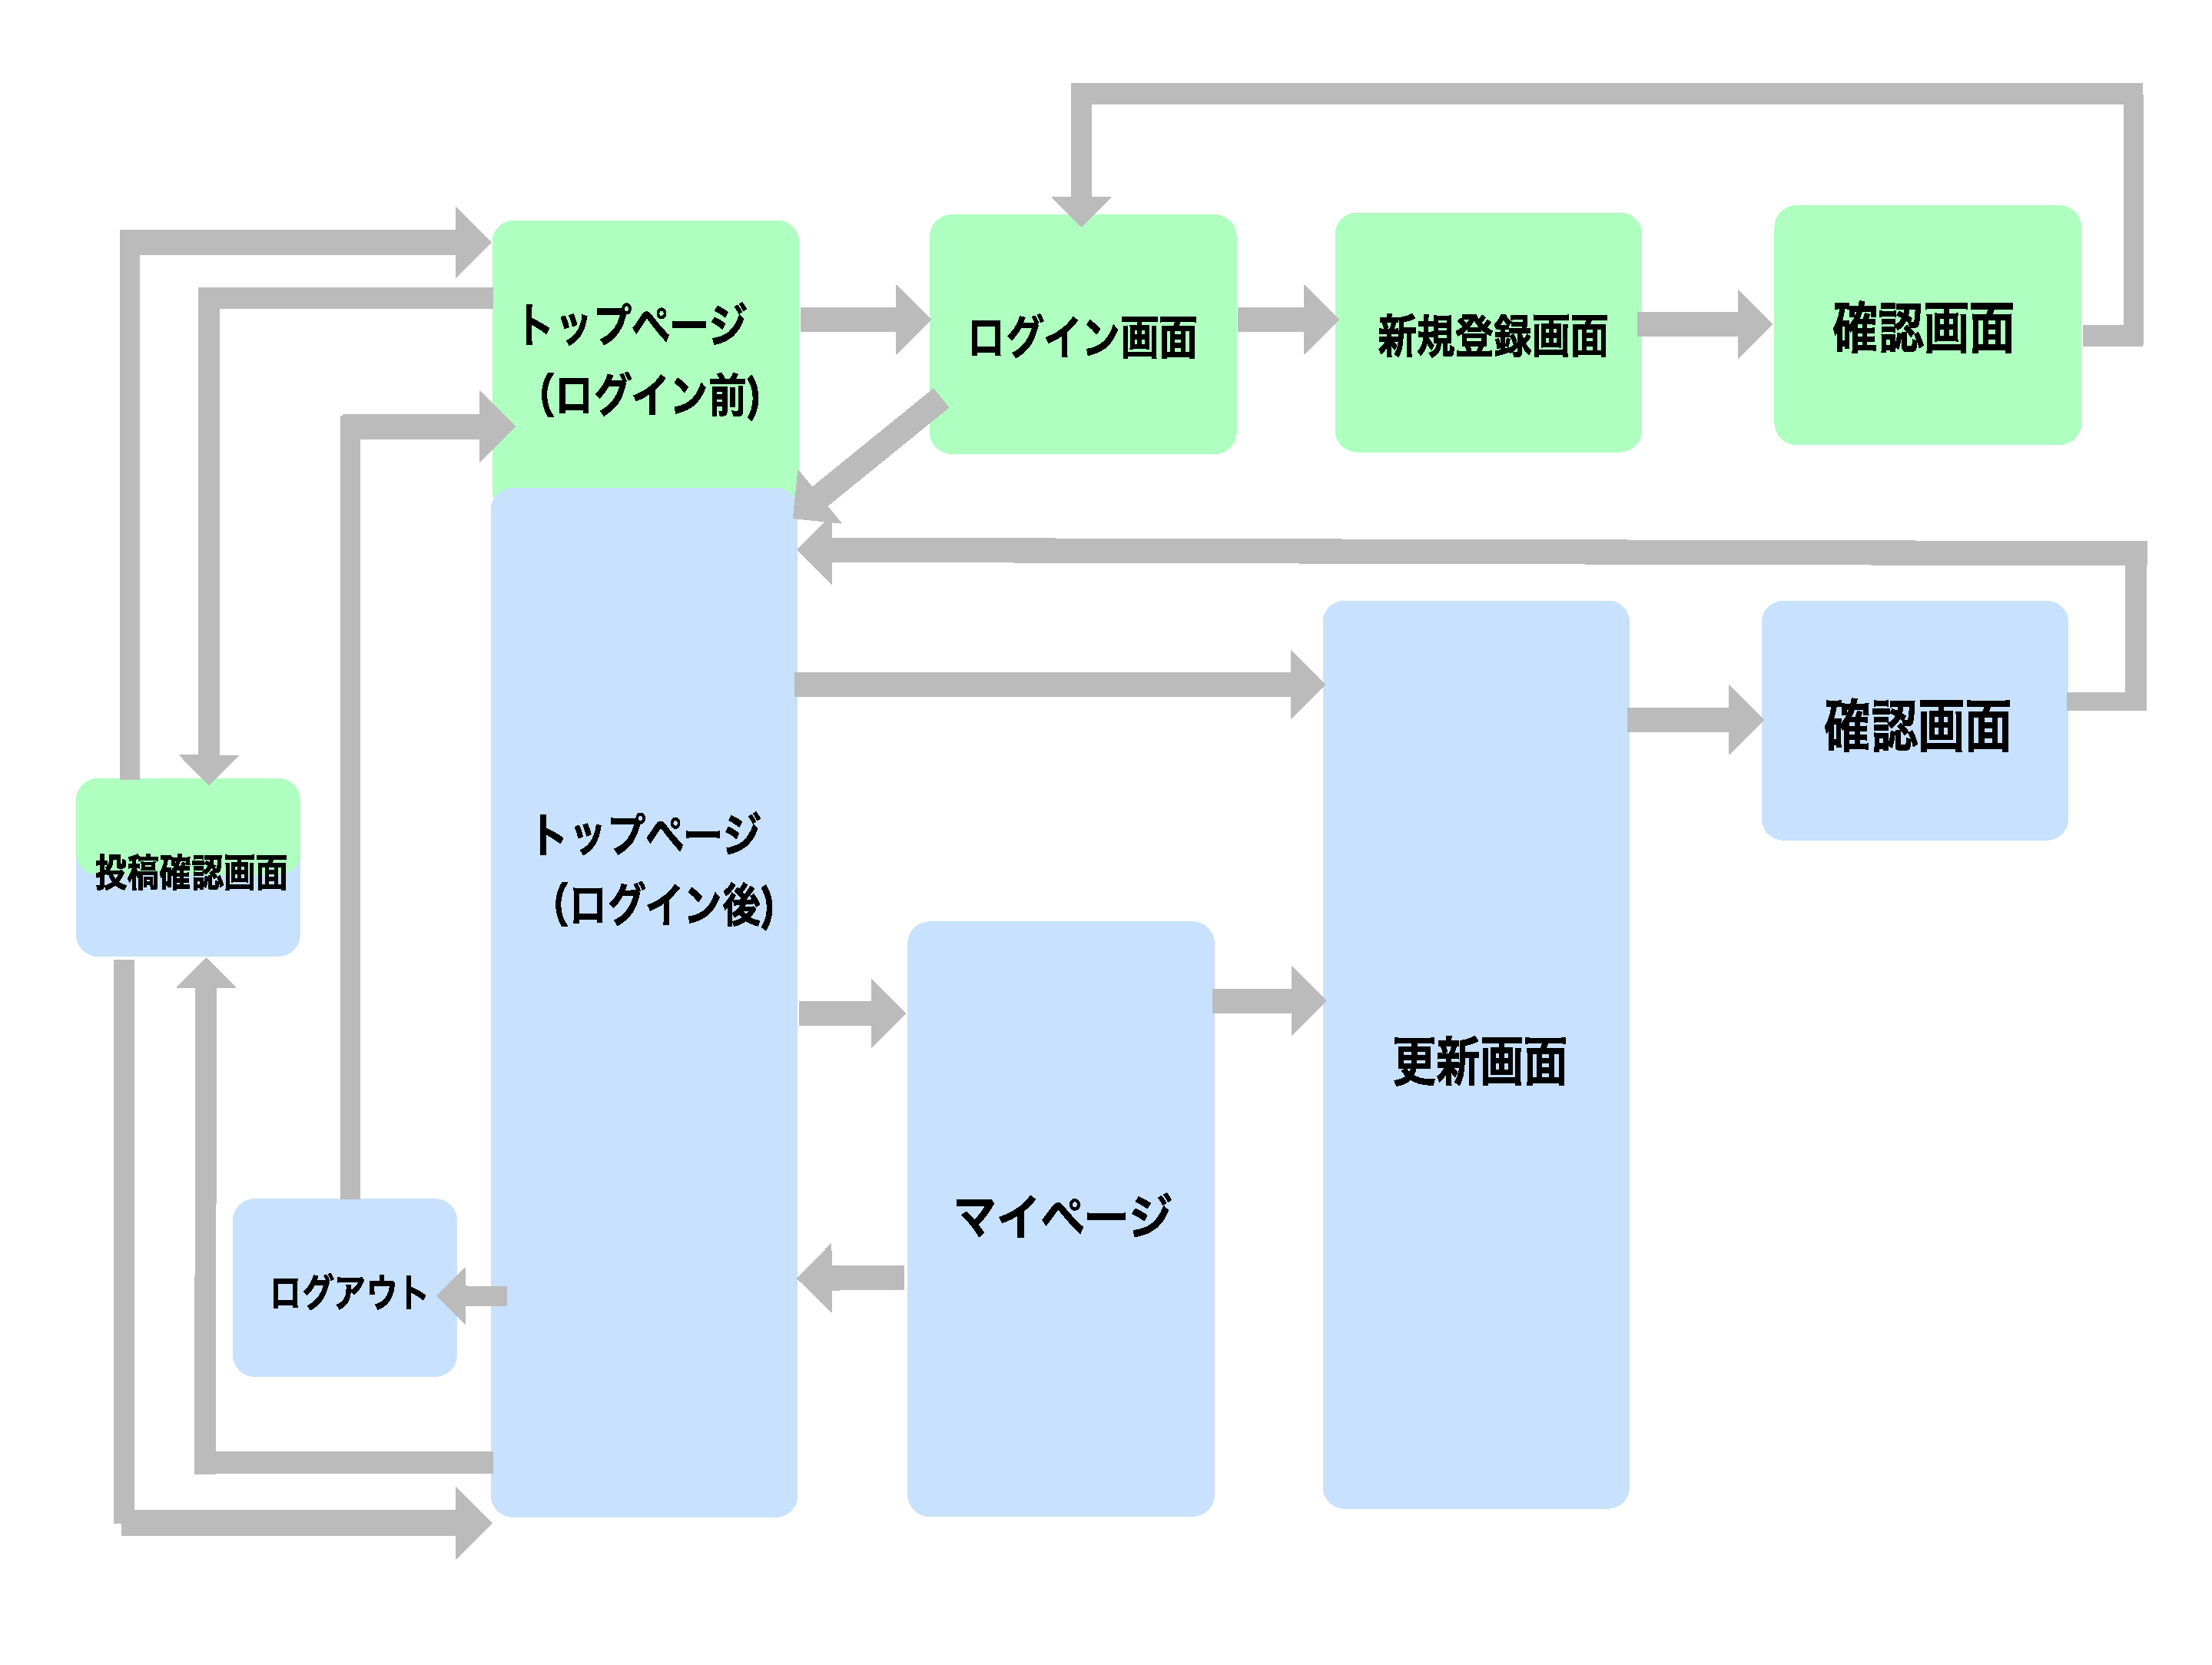
\includegraphics[scale=0.17]{systemScreen.eps}
\caption{状態遷移図}
 \label{システム}
\end{figure}

\subsection{データベース設計}
本システムで使用されているデータベースでは次の2つのテーブルが使われている. 
\begin{quote}
 \begin{itemize}
  \item ユーザ情報テーブル
  \item 備忘録テーブル
 \end{itemize}
\end{quote}

まずユーザ情報テーブルの構成は表1のようになっている. 個々の識別用のemailカラム, ユーザネームを格納するuser\_nameカラム, パスワードを格納するpasswordカラムがこのテーブルでは使用されている. 
またメールアドレスとパスワードはともに128文字, ユーザネームは50文字の領域が割り当てられている. どちらも指定文字数を超えるとエラーが出るようになっているので格納時の例外は出ることはない. 

\begin{table}[htb]
\centering
  \caption{ユーザ情報テーブル構成}
  \scalebox{0.7}{
  \begin{tabular}{|l|c|r|c|c|c|}  \hline
    	Field & Type & Null & Key & Default & Extra \\ \hline \hline
   	 id & int(10) unsigned & NO & PRIMARY & NULL & auto\_increment \\ \hline
	 email & varchar(128) & NO & UNIQUE & NULL & \\ \hline
	 user\_name & varchar(50) & NO & & NULL & \\ \hline
	 password & varchar(128) & NO & & NULL & \\ \hline
   	\end{tabular}
   }
\end{table}

次に備忘録テーブルである. 備忘録テーブルの構成は表2のようになっている. 投稿時の西暦から秒数までの時間を格納するcreated\_atカラム, タイトルを格納するsubjectカラム, 本文を格納するtextカラム, 誰が投稿したかのユーザidを格納するuser\_idカラム, プライベート投稿であるかの真偽が格納されているis\_privateカラムがこのテーブルで使用されている. 
また, subjectカラムは100文字, textカラムは500文字の領域が割り当てられている. 本文であるtextカラムは400文字までという制限が設けられているが, 念のため余分に領域を割り当てている. 
is\_privateカラムでは1bitのtinyint型が付けられているのでこの値が1か0かでプライベート投稿であるかをチェックしている. 

今回はLaravelを使用しているのでテーブル同士の関連づけが簡単にできるようになっている. よってuser\_idに格納されたidのユーザを参照してこの備忘録が誰によって投稿されたものなのかを表示している. この機能はマイページでの表示にも使われている. 

\begin{table}[htb]
\centering
  \caption{備忘録テーブル構成}
  \scalebox{0.7}{
  \begin{tabular}{|l|c|r|c|c|c|}  \hline
    	Field & Type & Null & Key & Default & Extra \\ \hline \hline
   	 id & int(10) unsigned & NO & PRIMARY & NULL &  auto\_increment \\ \hline
	 created\_at & timestamp& NO & & current\_timestamps() & \\ \hline
	 subject & varchar(100) & NO & & NULL &  \\ \hline
	 text & varchar(500) & NO & & NULL &  \\ \hline
	 user\_id & int(11) & YES & & NULL &  \\ \hline
	 is\_private & tinyint(1) & NO & & NULL &  \\ \hline

   	\end{tabular}
   }
\end{table}

\subsection{システム詳細}
前述の通り, 今回はLaravelを使用しているのでMVC方式でファイルを分けて構成されている. このシステムで主に働いているファイルは以下の通りである. 

\begin{quote}
 \begin{itemize}
  \item コントローラ
   \begin{itemize}
   \item SimpleNoteController.php
   \item UserController.php
   \item NoteController.php
   \end{itemize}
  \item モデル
   \begin{itemize}
    \item User.php
    \item Notebook.php
   \end{itemize}
  \item ビュー
   \begin{itemize}
    \item index.blade.php
    \item login.blade.php
    \item register.blade.php
    \item registerConfirm.blade.php
    \item registerComplete.blade.php
    \item editUser.blade.php
    \item editConfirm.blade.php
    \item editComplete.blade.php
    \item mypage.blade.php
    \item uploadConfirm.blade.php
    \item template.blade.php
   \end{itemize}
   \item リクエストクラス
   \begin{itemize}
    \item EditRequest.php
    \item RegisterRequest.php
    \item UploadRequest.php
   \end{itemize}
 \end{itemize}
\end{quote}

SimpleNoteControllerクラスでは特に深くデータベースとの連携がない処理を行っているのでindexメソッドやloginメソッド, registerメソッドではそのままトップページや登録画面を表示するのみとなっている. また, regist\_confirmメソッドでは新規登録の確認画面の際にhtmlの方に表示するデータの転送とセッションへの格納により入力したデータを確認として表示させている. 

またlogoutメソッドではセッションに格納してあるログインIDとユーザネームを消してリダイレクトすることでログアウト機能を実現している. 

UserControllerクラスではユーザ情報をモデルとビュー間でやり取りする処理が行われている. regist\_completeメソッドではユーザ情報をデータベースに格納させる処理を行っている. 前ページからセッションで受け取ったユーザデータにバリデーションを行ったのちにユーザネームとメールアドレス, さらにパスワードをハッシュ化した状態で格納させている. 
そしてlogin\_checkメソッドではログイン時のデータチェックを行っている. データベース内から入力メールアドレスと登録メールアドレスを比較して一致したものがない, またはメールアドレスは一致していたとしてもパスワードが一致していない場合はその趣旨のエラーをビューに返すようにしている. 

editメソッドは登録情報を編集する際に入力フォームに登録データを入力しておくために呼び出され, edit\_confirmメソッドでregist\_confirmメソッドと同じく確認画面のためのデータ転送, セッションへの格納を行っている. そしてedit\_completeメソッドで入力された変更情報を再挿入している. 

NoteControllerクラスでは備忘録情報をモデルとビュー間でやり取りする処理が行われている. uploadメソッドではトップページで入力された備忘録情報を受け取り, プライベート投稿であるかのフラグをbooleanに変換した状態でセッションに格納した上で確認画面に飛ばしている. 
そしてupload\_completeメソッドで実際に入力されたデータをデータベースに格納するという仕組みになっている. ユーザデータの格納と違うところはプライベート投稿であるかのbooleanを判別する部分のみで他はほとんど同じとなっている. そしてmypageメソッドではマイページで表示する備忘録の条件指定を行っている. 現在ログインしているユーザのIDのみで条件を絞り, 降順で表示させることで自分の投稿のみを表示させるようにしている. 

Userモデルクラスでは自動繰上げであるidカラムの保護, notebooksテーブルが従テーブルであることの宣言, バリデーションを指定している. 
また, Notebookモデルクラスでは自動繰上げ, 自動更新であるidカラムとcreated\_atカラムの保護, usersテーブルが主テーブルであるのことの宣言, 同じくバリデーションを指定している. 

リクエストクラスは確認画面に飛ぶ前に入力情報が条件に合っているかのバリデーション機能を使用するために実装している. 今回は新規登録, 登録情報の変更, 備忘録の投稿の際にバリデーションを使用しているので, regist\_confirmメソッドではRegisterRequestクラスを呼び出して新規登録時のバリデーション, edit\_confirmメソッドではEditRequestクラスを呼び出して登録情報変更時のバリデーション, uploadメソッドではUploadRequestクラスを呼び出して備忘録投稿時のバリデーションを行って, 機能ごとそれぞれのバリデーションを実装している. 

\subsection{変数設計}

今回はセッション変数とPOST変数を多く使用してデータのやり取りをしている. ここで使用されている変数の一覧は以下のようになっている. 

\begin{quote}
 \begin{itemize}
  \item セッション変数
   \begin{itemize}
    \item *user\_name : ユーザネームの格納
    \item *mail : メールアドレスの格納
    \item *password : パスワードの格納
    \item login\_id : ログインしているユーザIDの格納
    \item login\_user : ログインしているユーザネームの格納
    \item *title : 備忘録の件名の格納
    \item *texts : 備忘録の本文の格納
    \item *isPrivate : プライベート投稿であるかのフラグの格納
   \end{itemize}
  \item POST変数
   \begin{itemize}
    \item user : ユーザネームの格納
    \item mail : メールアドレスの格納
    \item pass : パスワードの格納
    \item isLoginError : ログインエラーである時のフラグの格納
    \item notes : 備忘録データの格納
    \item title : 備忘録の件名の格納
    \item texts : 備忘録の本文の格納
    \item isPrivate : プライベート投稿であるかのフラグの格納
   \end{itemize}
 \end{itemize}
\end{quote}

また * マークの付いているセッション変数はLaravelの機能であるフラッシュデータと呼ばれるものであることを示している. これは常にサーバに残り続ける通常のセッション変数とは違い, リダイレクト後に自動的にセッションから削除される一時的な変数である. 
このフラッシュデータを使用してデータベースに格納するデータを保存して格納完了後にセッションから消去されるようにしている. 

さらにlogin\_idはログインしている状態を保つために使用されており, login\_userは備忘録投稿の際のユーザ名の表示のために使用されている. なのでログアウトの際にはこれらの変数を削除することでログアウト機能を実装している. 

そしてPOST変数は主に新規登録, 登録内容の編集, 投稿の確認画面にデータを転送する際に使用されている. 
他にもnotesという全ての備忘録データをビューに転送する変数やisLoginErrorというログインエラーであった時のみ転送されるフラグ変数も導入されている. 

\section{実装}
\subsection{実装環境}
本システムの実装環境は以下の通りである. 

\begin{quote}
 \begin{itemize}
 \item MariaDB 10.4.21
 \item PHP 8.1.4
 \item Laravel 4.2.10
 \item Composer 2.3.9
 \end{itemize}
\end{quote}

\subsection{環境設定}
今回の開発ではXAMPPは一切使わずに全てLaravelで環境設定を行っている.
Laravelのenvファイルにデータベースやメールの設定を追記することで使用可能になる. 今回はmysqlでlocalhostを使用の上, ポート番号は3306, 使用データベースはsimple\_notebooks, ユーザネームはテスト用のユーザとしてginginを設定している. 

\subsection{動作検証}
ログインを完了させるまでの画面遷移は図3のようになっている. まずトップページのサイドメニューからログインを選ぶと, メールアドレスとパスワードを入力するフォームが表示されるので登録情報を入力することでログインが完了し, トップページに遷移する. 
また, 入力したユーザ情報が存在していなかったりメールアドレスやパスワードが間違っていたりすると「メールアドレスかパスワードが違います」と言ったエラーメッセージが表示される. 
\begin{figure}[h]
 \centering
 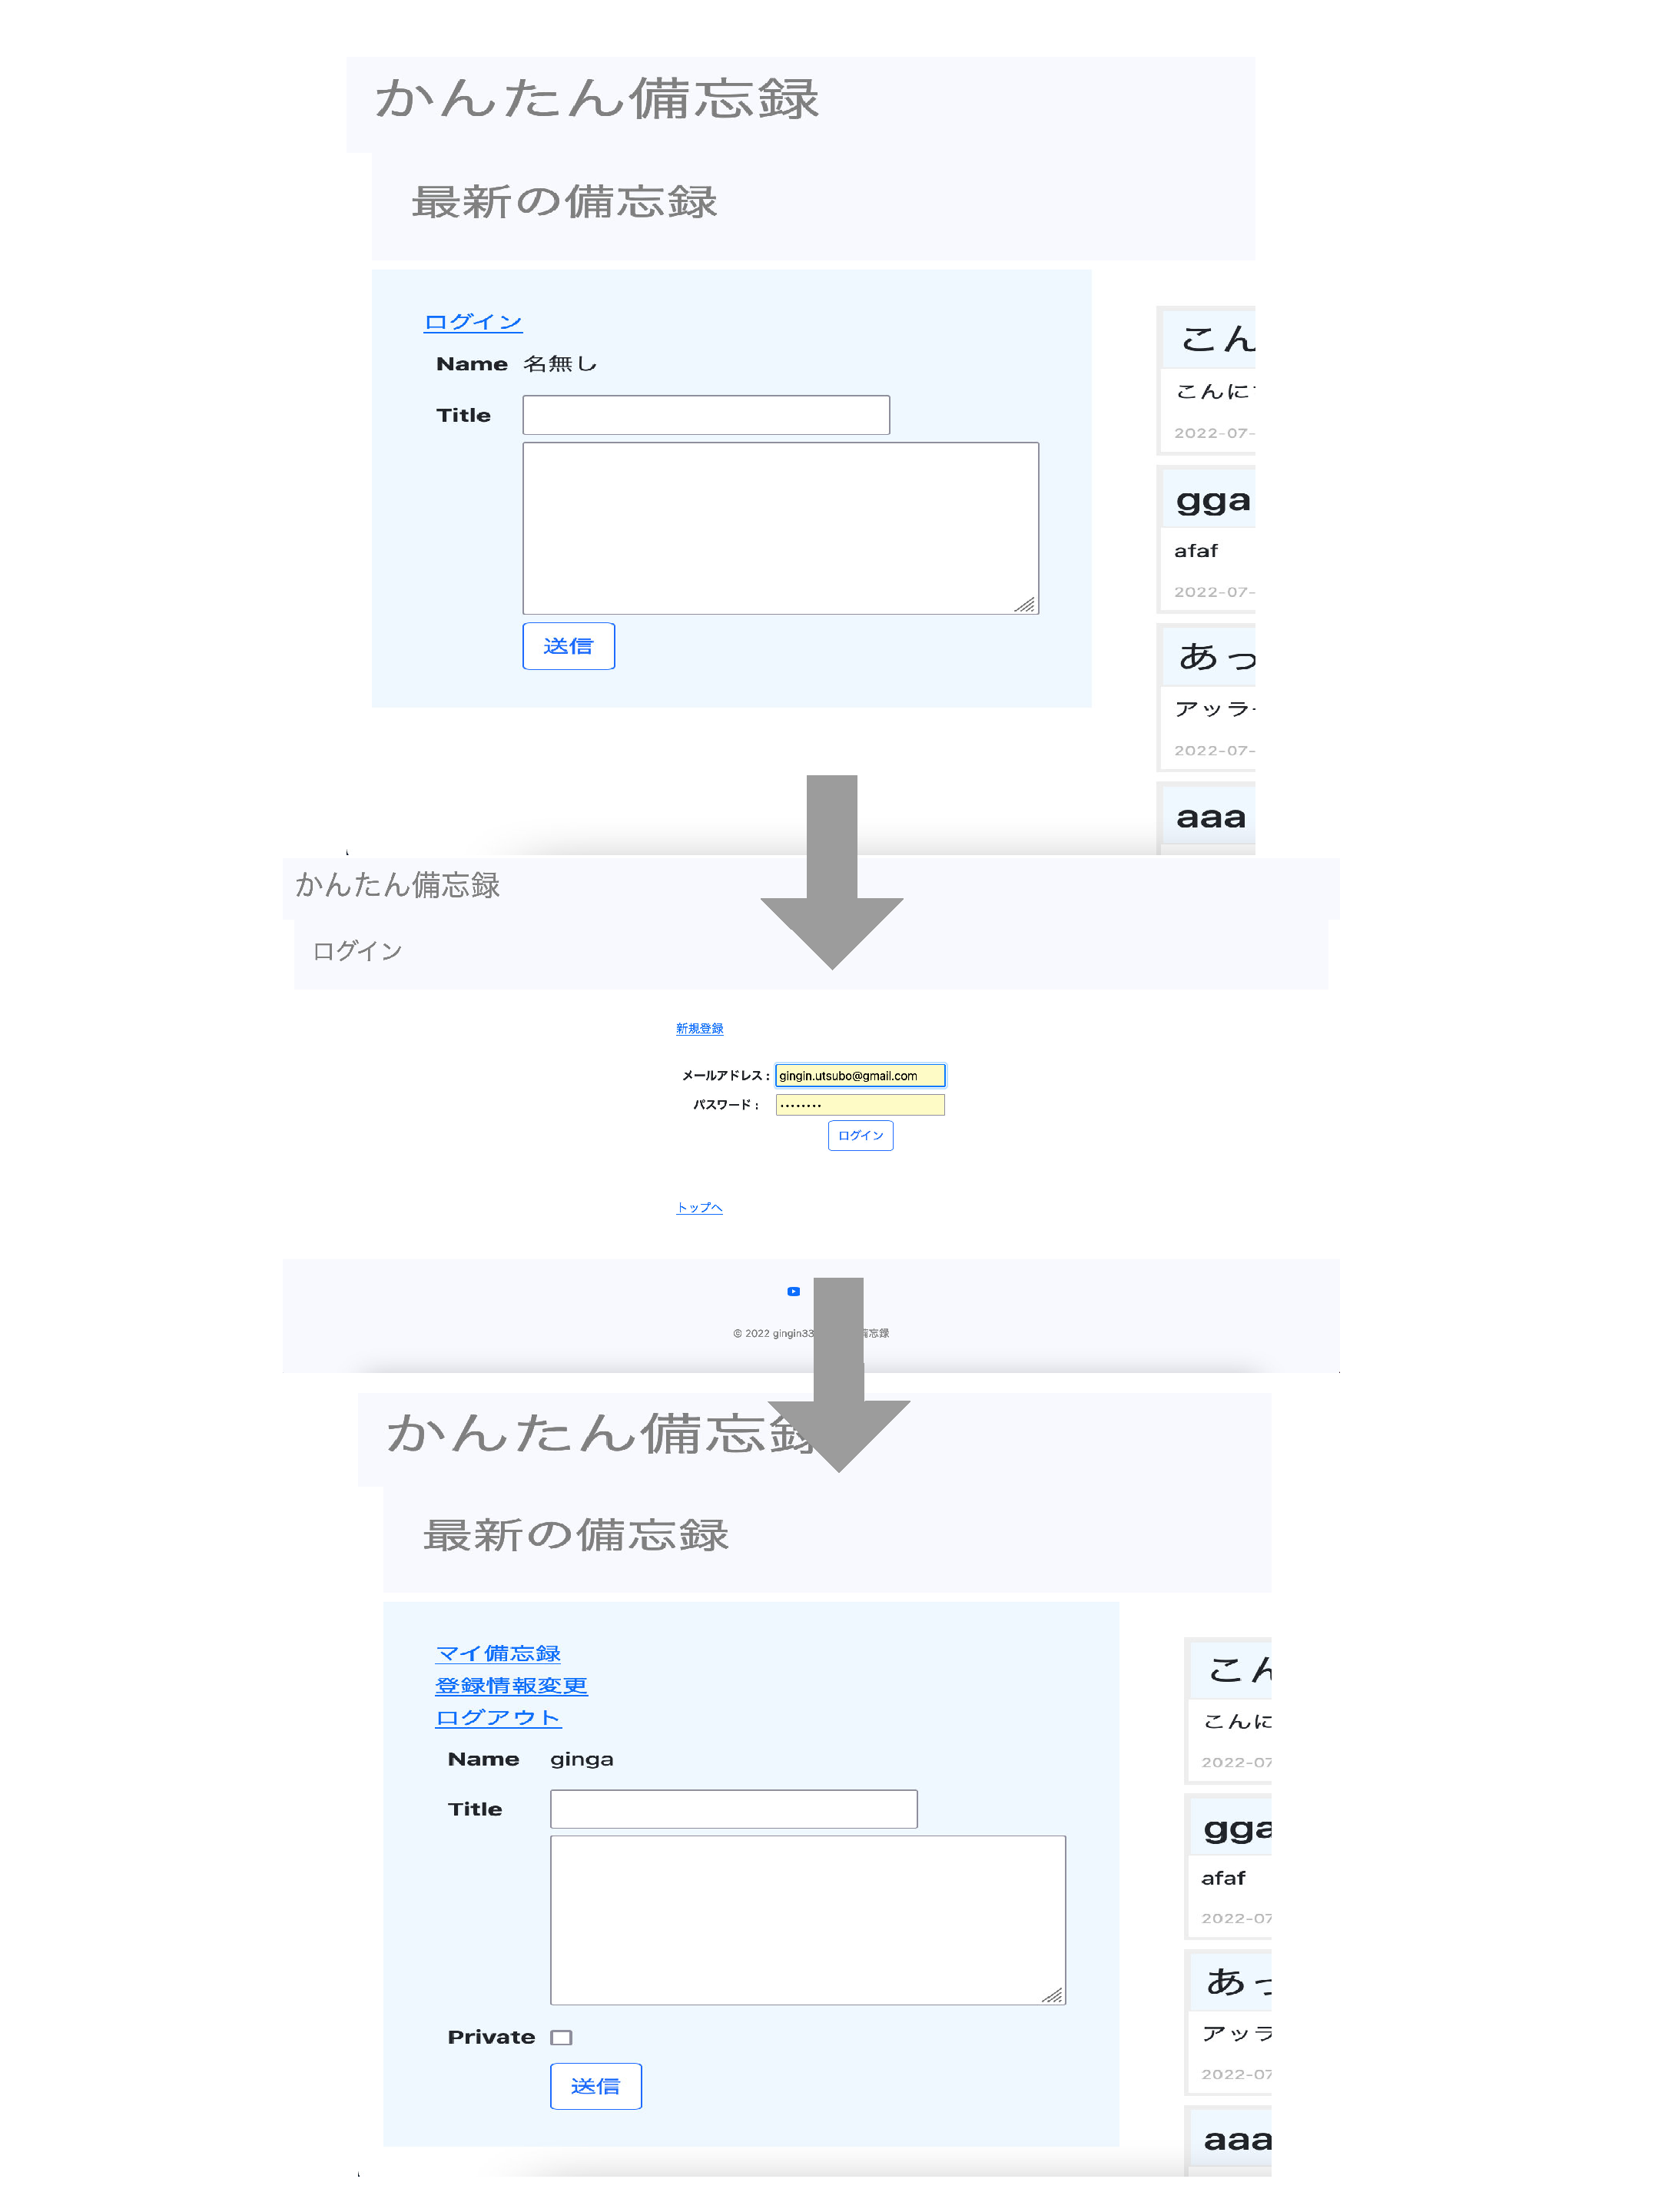
\includegraphics[scale=0.17]{toLogin.eps}
\caption{ログイン完了までの流れ}
 \label{ログインまで}
\end{figure}

そして備忘録の投稿を完了させるまでの画面遷移は図4のようになっている. トップページのサイドバーに入力フォームが設置されているので, 件名と本文を入力して送信すると確認画面に飛ぶことができ, そこから投稿完了となる. このときに件名と本文が入力されていなければその趣旨のエラー文が表示される. 

\begin{figure}[h]
 \centering
 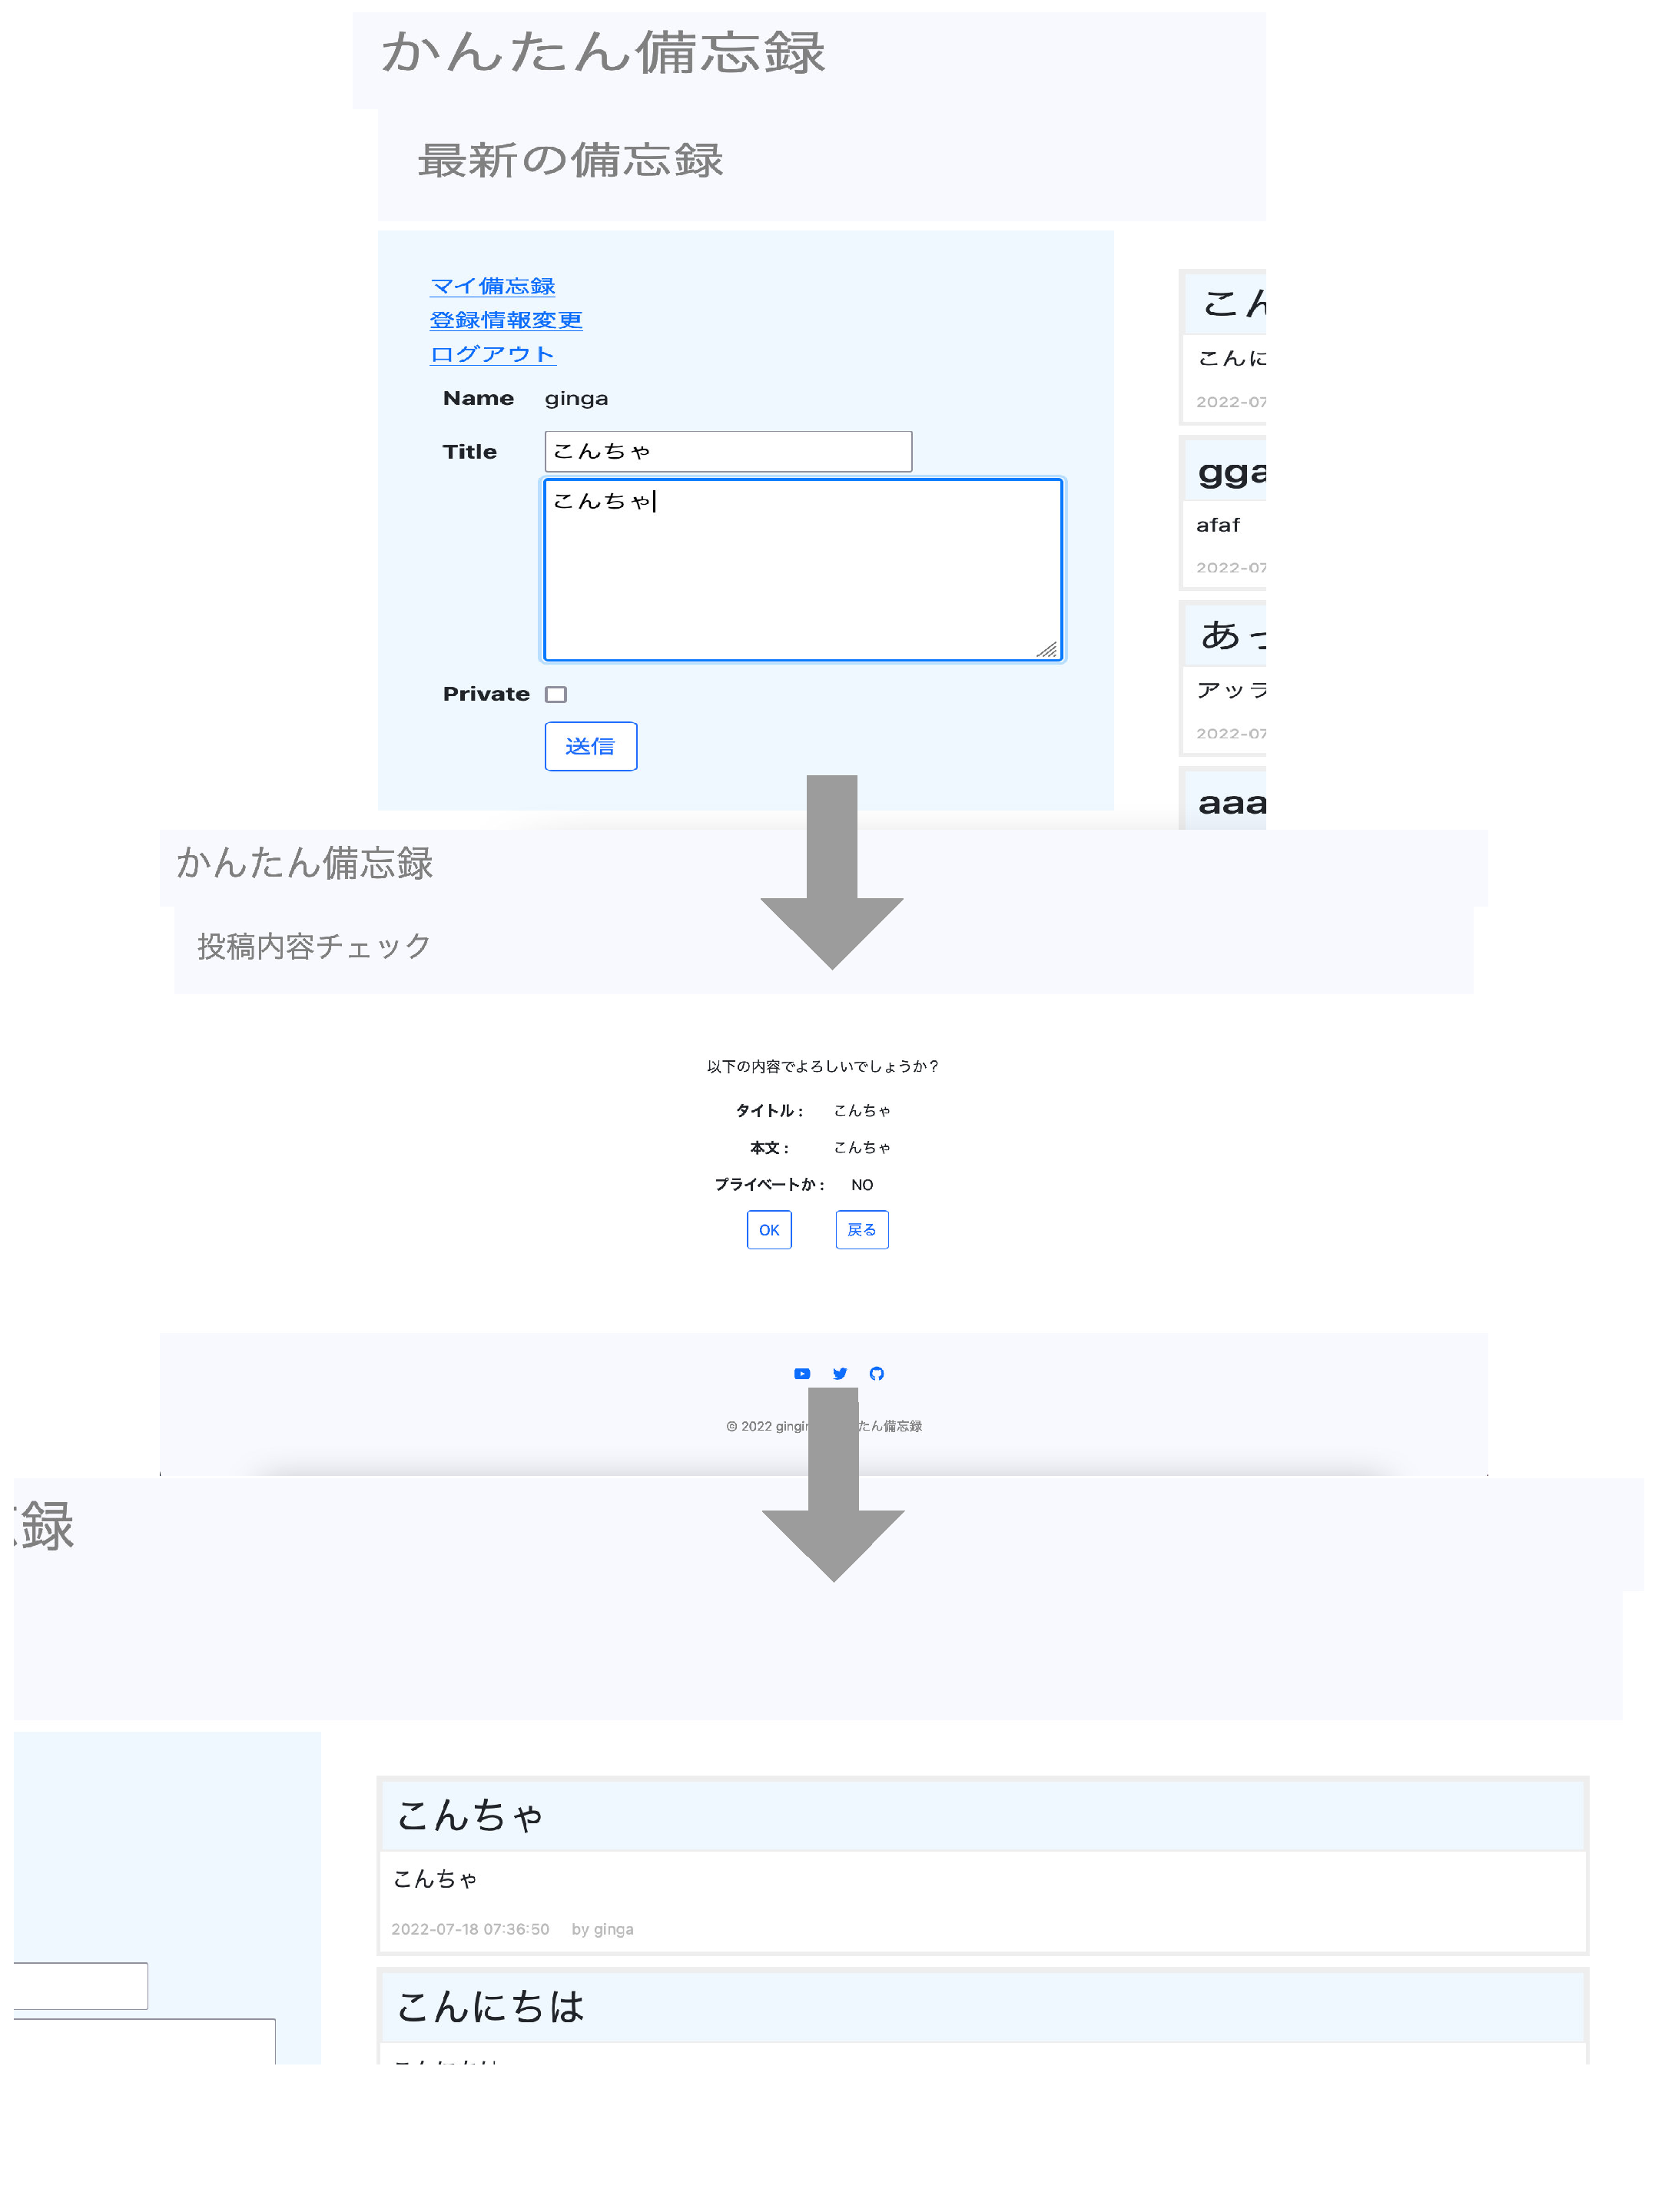
\includegraphics[scale=0.17]{toUpload.eps}
\caption{備忘録投稿完了までの流れ}
 \label{投稿まで}
\end{figure}

最後に新規登録完了までの画面遷移は図5のようになっている. 
ログイン画面の左上のリンクから新規登録をすることができる. ユーザネームとメールアドレス, パスワードと確認用のパスワードを入力することで登録情報の確認画面に遷移することができる. 
この際, パスワードが8文字未満であったり, メールアドレスがアドレスの形式でない, またこれらが入力されていない場合はこの場でエラー文が表示される. 確認が終わり, 次に進めば新規登録完了となり, 登録した内容でログイン可能となる. 

\begin{figure}[h]
 \centering
 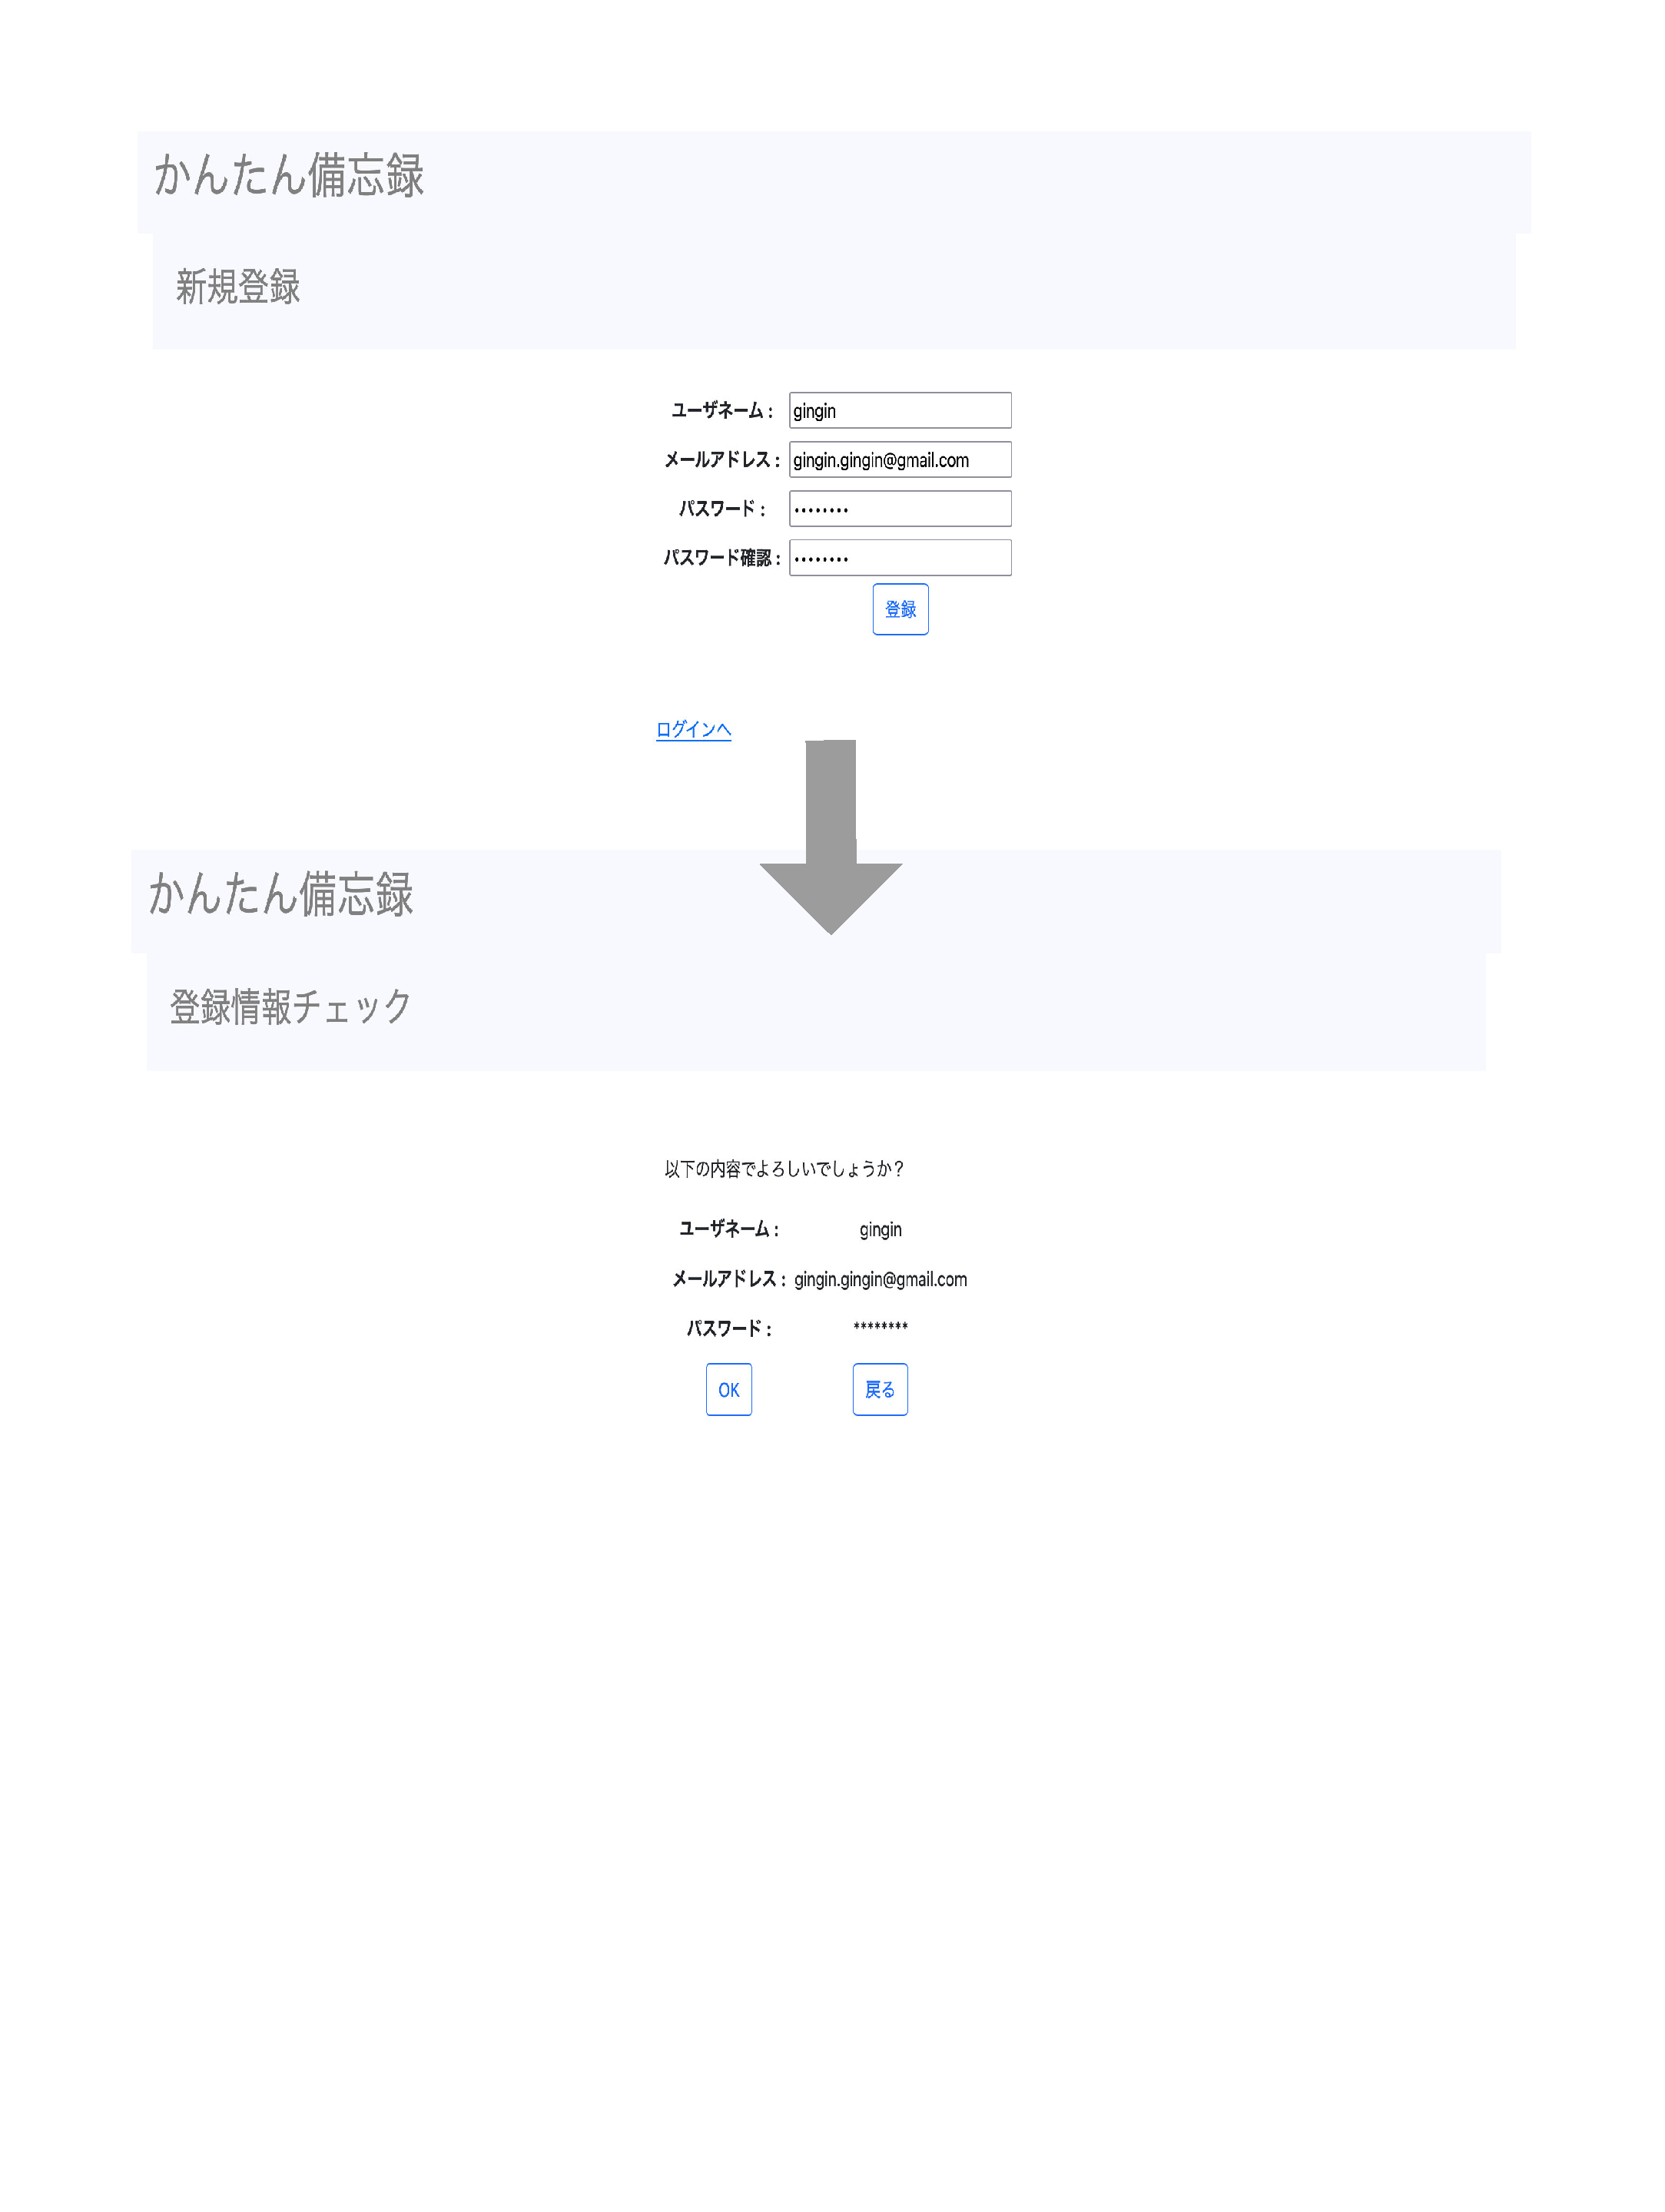
\includegraphics[scale=0.17]{toRegist.eps}
\caption{新規登録完了までの流れ}
 \label{登録まで}
\end{figure}

\section{まとめ}

今回はかんたん備忘録というシンプルなTODOWebアプリケーションを作成した. Laravelについて勉強しながら同時に制作したが, 思い通りの動作をさせることができた. 
この制作でLaravelについての理解をさらに深めることができ, 今後のWebアプリケーションの制作にも活かせると考えたので大きな勉強になった. しかしその反面, Laravelの認証などの様々な機能を完全に使いこなすことはできなかったので今後制作するときはしっかり学んだ上で作りたい. 


\begin{thebibliography}{9}
\bibitem{php} PHP Group . "一般的な情報" . php. https://www.php.net/manual/ja/faq.general.php . (閲覧日:2022/05/29)
\bibitem{php} PHP Group . "Zend API: PHP のコアをハックする" . php . http://php.adamharvey.name/manual/ja/internals2.ze1.zendapi.php . (閲覧日:2022/05/29)
\bibitem{php} PHP TUTORIAL . "What is PHP" . phptutorial.net . https://www.phptutorial.net/php-tutorial/what-is-php/ (閲覧日:2022/05/29)
\bibitem{mysql} KINSTA . "MySQLとは?初心者にわかりやすい説明" . KINSTA . (更新日:2020/07/03) . https://kinsta.com/jp/knowledgebase/what-is-mysql/ . (閲覧日:2022/06/01)
\bibitem{mariaDB} MariaDB Foundation . "MariaDB Server: The open source relational database" . MariaDB Foundation . https://mariadb.org/ . (閲覧日:2022/06/01)
\bibitem{mariaDB} Mark Smallcombe . "MariaDB vs MySQL: 徹底比較" . integrate.io . (更新日:2020/09/03) . https://www.integrate.io/jp/blog/mariadb-vs-mysql-everything-you-need-to-know-ja/ . (閲覧日:2022/06/01)
\bibitem{css} MDN contributors . "CSS: カスケーディングスタイルシート" . mdn web docs . (更新日:2021/07/18) . https://developer.mozilla.org/ja/docs/Web/CSS . (閲覧日:2022/06/01)
\bibitem{laravel} Tutorials Point . "Laravel Overview" . tutorialspoint simply easy learning . https://www.tutorialspoint.com/laravel/laravel\_overview.htm . (閲覧日:2022/07/08)
\bibitem{http} MDN contributors . "HTTP" . mdn web docs . (更新日:2021/09/18) . https://developer.mozilla.org/ja/docs/Web/HTTP . (閲覧日:2022/06/01)
\end{thebibliography}


\end{document}
